\documentclass[12pt,a4paper]{amsart}
\usepackage[utf8]{inputenc}
\usepackage{amsmath}
\usepackage{amsfonts}
\usepackage{amssymb}

\usepackage{hyperref}

\usepackage{float}
\usepackage{subfig}


%\usepackage[dvipdfmx]{graphicx}
\usepackage{graphicx}
\usepackage{caption}
%\usepackage[nobysame, alphabetic]{amsrefs}
%\usepackage{here}
%\usepackage{showkeys}
\newcommand{\modif}{$\clubsuit$}
\newtheorem{thm}{Theorem}[section]
\newtheorem{defn}[thm]{Definition}
\newtheorem{coro}[thm]{Corollary}
\newtheorem{prop}[thm]{Proposition}
\newtheorem{lem}[thm]{Lemma}
%\theoremstyle{definition}
\newtheorem{rmk}[thm]{Remark}
\newtheorem{cond}[thm]{Condition}

%CB defs
\def\HH{\mathbb{H}}
\def\dHH{\partial \mathbb{H}}
\def\HHn{\HH^n}
\def\hd{\hat{\delta}}
\def\ha{\hat{\alpha}}
\def\haa{\ha \cup \{\alpha^+,\alpha^-\}}

\def\im{\mathrm{Im}\,}



\def\SL{\mathrm{SL}(2,\CC)}

\def\xx{\HH/g2}


\def\ZZ{\mathbb{Z}}
\def\CC{\mathbb{C}}
\def\RR{\mathbb{R}}
\def\QQ{\mathbb{Q}}
\def\NN{\mathbb{N}}

\def\tt{\Sigma_{1,1}}

\def\fp{\mathbb{F}_p}
\def\aut{\text{Aut}(\F2)}
\def\gl2{\mathrm{GL}(2, \ZZ)}
\def\sl2{\mathrm{SL}(2, \ZZ)}
\def\g2{\Gamma(2)}
\def\slc{\mathrm{SL}(2, \CC)}

\def\xx{\HH/\g2}
\def\gg{\mathcal{G}_n}
\def\ggp{\mathcal{G}_p}

\def\isom{\mathrm{isom}(\HH)}

\def\isomH{\text{isom}^+(\HH)}
\def\tr{\text{tr\,}}


\def\GI{\mathbb{Z}[i]}
\def\hc{\CC \setminus \GI}



\title{Geodesics and the sum of squares}

 \author[McShane]{Greg McShane}
 \author[Vlad]{Vlad Sergesciu}
\address{Institut Fourier 100 rue des maths, BP 74, 38402 St Martin d'H\`eres cedex, France}
\email{mcshane at univ-grenoble-alpes.fr}


\begin{document}

\maketitle

\begin{abstract} 
We prove Fermat's sum  of two squares theorem 
using well known calculations from hyperbolic geometry 
and considerations of automorphisms of the three punctured sphere.
\end{abstract} 


\section{Introduction}

Consider the following pair of well known theorems from elementary number theory:


\begin{thm}\label{triv}
Let $p$ be a prime then the equation
$$x^2 = -1$$
admits a solution in $\fp$ iff 
$p =2$ or $p-1$ is a multiple of $4$.
\end{thm}


\begin{thm}[Fermat]\label{main}
Let $p$ be a prime then the equation
$$x^2 + y^2 = p $$
has a solution in integers  iff  $p =2$ or $p-1$ is a multiple of $4$.
\end{thm}

These results are intimately linked and often one deduces the second as a corollary of the first,
 for example, by using unique factorisation in the Gaussian integers.  We present a unified geometric  approach to these results  using the theory of group actions and in particular an application of Burnsides's Lemma. 
 
 
As in Zagier's remarkable proof \cite{zagier} both results follow from showing that a certain involution has a fixed point. Amusingly Burnsides's Lemma reduces this to showing that another involution has exactly two fixed points:
\begin{itemize}
\item  In the proof of Theorem \ref{triv} this is a consequence of the fact that a quadratic equation 
over a field has at most two solutions.
\item In the proof of Theorem \ref{main} this follows from some geometry and the fact that 
$$ \det 
\begin{pmatrix}
k + 1 & k- 1\\
p & p 
\end{pmatrix} = 2p \neq 2.
$$
 \end{itemize}


\subsection{Organisation, Remarks}

In Section 2 we recall the statement of Burnsides Lemma 
and apply it to a Klein four group generated by involutions of $\fp^*$
yielding a proof of Theorem \ref{triv}. In Section 3 we introduce $\g2$
and the associated Riemann surface $\xx$. 
In Section 4, for each prime $p$
we study how the automorphisms of $\xx$ 
act on a family of geodesic on this surface
obtained in a natural way from the rationals $k/p$.
In particular we show (Lemma \ref{the end})  that if $p$ is congruent to 1 modulo 4
there is always an orientation preserving involution that
leaves one of our geodesics invariant
and from this we deduce Theorem \ref{main}.

\subsubsection{References}
Almost all  of the material in Sections 3 and 4 
can be found in Serre's book \cite{serre} and the reader
should not need any other references to understand 
this paper if they are already familiar with  Burnsides Lemma.

\subsubsection{Burnside and signatures}
 The astute reader will surely realise that Burnside is not essential to our argument
 and that one can achieve the same reduction by considering the signature
 of the permutations associated to the  involutions we consider. 
 In fact the first author set this as an  undergraduate exam question some years ago.
 
 \subsubsection{Farey tessalation}
 The argument in Lemma \ref{the end} is inspired by the definition of the 
 \textit{Farey tessalation}.
 
  \subsubsection{Lambda lengths}
 The idea of associating a length to a geodesic joining cusps
 (paragraph \ref{lengths}) appears in Penner's work on moduli \cite{bob}.
He defined the $\lambda$-length of simple bicuspidal geodesic 
on a punctured
surface to be the length of the portion outside of some fixed
 system of cusp regions.
 
 By using calculations in Wolpert \cite{saw}
 one can show that, for a suitable choice of cusp region 
 on the modular torus  the $\lambda$-lengths of arcs 
 coincide with the squares of Markoff numbers. 
 Then, using the fact that each arc is invariant under the 
 elliptic involution one can show, 
using Lemma \ref{squares},
 that every Markoff number is the sum of two squares.
 In fact this was the observation that was the starting point for this paper.
 
 \subsubsection{Bezouts Theorem}
 We are implicitly using  Bezout's Theorem
 (and in particular in the proof of Lemma \ref{action})
 when we assert that
 \begin{itemize}
 \item $\sl2$ is transitive on $\QQ \cup \infty$ (which is equivalent to Bezout's Theorem.)
 \item $\g2$ has exactly three orbits on $\QQ \cup \infty$.
 \end{itemize}
In fact Lemma \ref{action} can be proved
 without using our notion of length for a bicuspidal geodesics 
 but  instead by studying the action of 
 the lifts $U'$, $V'$  of the generators of our group $K^0$  
 and applying Bezout's Theorem.
 

\subsection{Thanks}

The first author thanks Louis Funar and the second author for  many useful
conversations over the years concerning this subject. He would also like to
thank Xu Binbin for reading early drafts of the manuscript.


\section{Burnside Lemma}

We give a proof of Theorem \ref{triv} using the Burnside Lemma.
Recall that if $G$ is  a group acting on a finite set $X$ then the Burnside Lemma says
\begin{equation}\label{burnside}
|G| |X/G| = \sum_{g} |X^g| 
\end{equation}  
where, as usual, 
 $X^g$ denotes the set of fixed points of the element $g$ 
 and $X/G$  the orbit space.


Let $p\neq 2$,  $X = \fp^*$ and $G$ be the group generated by the two involutions
\begin{eqnarray*}
x & \mapsto -x \\
x & \mapsto 1/x.
\end{eqnarray*}
The group  $G$ has exactly four elements namely:
\begin{itemize}
\item the trivial element which has  $p-1$ fixed points
\item $x\mapsto -x$ which has no fixed points 
\item  $x\mapsto 1/x$ has exactly two fixed points namely $1$ and $-1$.
\item  $g:x \mapsto -1/x$ is the remaining element and the theorem is equivalent to the existence of a fixed point for it.
\end{itemize}
Note that since $\fp$ is a field 
$|X^g| = \sharp \{x^2 = -1, \, x\in \fp^* \}$
is either $0$ or $2$.
Now for our choice of $X$ and $G$ equation (\ref{burnside}) yields
\begin{equation}
4 |X/G|   = (p-1) + 2 + |X^g|.
\end{equation}  
The LHS is always divisible by $4$ so the  RHS is too and
it follows from this that
$$ |X^g|. = \left\{  \begin{array}{ll}
0 & (p-1) =  2 \mod 4 \\
2 & (p-1) =  0 \mod 4 \\
\end{array}
\right.
$$
This proves Theorem \ref{triv}.

\subsection*{Note}
As was noted in the introduction one can obtain the same conclusion 
by calculating the signature of $x\mapsto -1/x$ 
using the fact that it is  the composition of
$x \mapsto -x$ and $x \mapsto 1/x$.


\section{Automorphisms of the three punctured sphere}


We consider $\g2$,
the principal level 2 congruence subgroup of $\sl2$.
This group acts on $\ZZ^2$, that is pairs of integers,  preserving parity.
It also acts on $\HH$ by linear fractional transformations
that is:
$$\begin{pmatrix}
a & b \\
c & d
\end{pmatrix} \in \sl2,\, z\in \HH,\, 
\begin{pmatrix}
a & b \\
c & d
\end{pmatrix}. z = \frac{az + b}{cz + d}.
$$
The quotient $\xx$ is conformally equivalent to the Riemann  sphere minus three points
which we will refer to as \textit{cusps}
(see Figure \ref{3punctured}). 
Following  convention we label these cusps $0,1,\infty$ respectively
corresponding to the three $\g2$ orbits of $\QQ \cup \infty$. 
Finally, the \textit{standard fundamental domain}  for $\g2$ 
is the convex hull of the points $\infty, -1, 0 , 1$.
This region can be decomposed into two ideal triangles 
$\infty, -1, 0 $ and $ 0 , 1,\infty$ as in Figure \ref{fund}.
The edges of the ideal triangles project to three disjoint simple geodesics on $\xx$
and each edge has a \textit{midpoint} 
which is a point of the $\sl2$ orbit of $i$ (see Figure \ref{3punctured}).

 \begin{figure}[hb]
\begin{center}
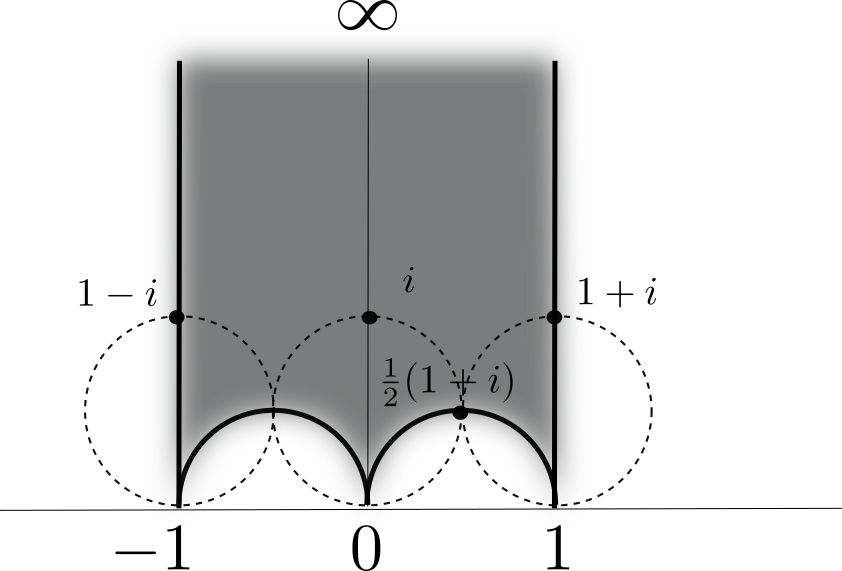
\includegraphics[scale=.5]{fund_dom.png} 
\end{center}
\caption{Standard fundamental domain for $\g2$ and its decomposition into ideal triangles.}
\label{fund}
\end{figure}


\subsection{Automorphism groups}
From covering theory an isometry  of $\HH$ 
induces an automorphism of $\xx$ iff it normalises the covering group
i.e. $\g2$.
It follows that,
since $\g2$ is a normal subgroup of $\sl2$,
 the quotient group
$$H^+: = \sl2/\g2$$
acts as a group of (orientation preserving) automorphisms of the surface $\xx$.
More generally, $\g2$ is normal in $\gl2$ and 
$$H: = \gl2/\g2$$
acts as a group of possibly orientation reversing  automorphisms of the surface $\xx$.


\subsection{Orientation reversing automorphisms}
To prove Theorem \ref{main} we will have to work with automorphisms
that do not preserve the orientation and in particular 
those induced by the involutions:
\begin{eqnarray*}
U: z &\mapsto& -\bar{z} \\
V: z &\mapsto& 1 -\bar{z}.
\end{eqnarray*}
Both $U$ and $V$ normalise $\g2$ so induce automorphisms of $\xx$.
In fact, since $V$ is the composition of $U$ and $z \mapsto z + 1$,
it suffices to show that $U$ normalises $\g2$.
This is easy to check, for if  $a,b,c,d \in \ZZ$ 
and  $f(z) = (az + b)/ (cz +d )$  then one has:
$$ U\circ f \circ U^{-1} (z) =  -\overline{f(\bar{-z})} = -f(-z) =   \frac{az - b}{-cz +d }, $$
  so conjugation does not change the parity of $a,b,c,d$ 
  and it follows that  $U$ normalises $\g2$.


 \begin{figure}[hb]
\begin{center}
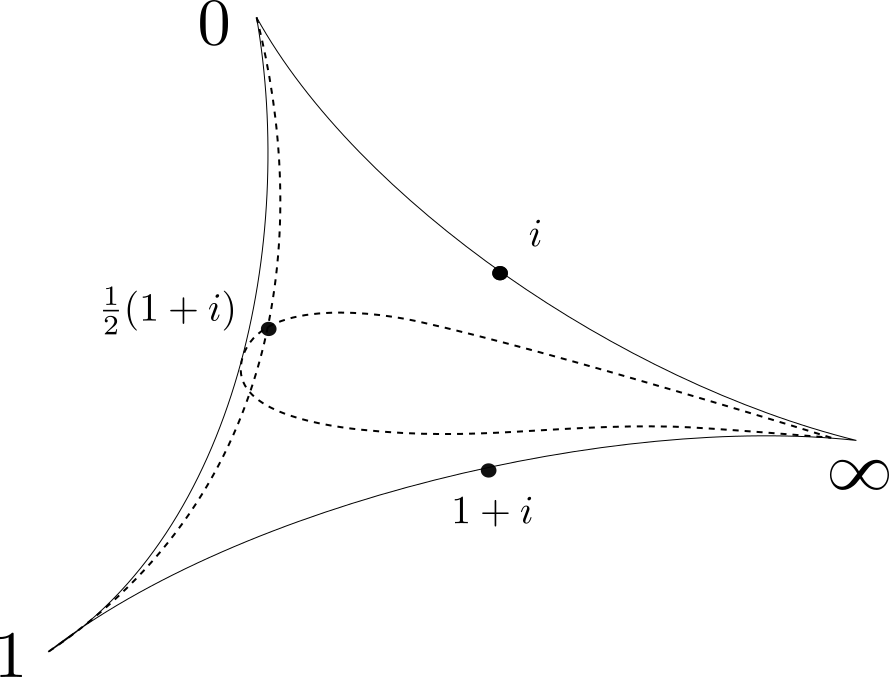
\includegraphics[scale=.5]{3sphere_again.png} 
\end{center}
\caption{Three punctured sphere with cusps and midpoints labelled.
The dotted loop is the fixed point set of the automorphism induced by $V$.}
 \label{3punctured}
\end{figure}



\subsection{Another Klein four group.}

The pair of involution $U,V$ generate a group 
of isometries of $\HH$,  which we denote by $\hat{K}^\infty$, 
 isomorphic to the infinite dihedral group $D_\infty$
infinite dihedral group. One checks that 
$$U\circ V (z) = V \circ U (z) = z + 1$$
and we note that 
$$  z + 1 = \frac{z+ 1}{ 0 + 1} = \begin{pmatrix}
1 & 1 \\ 0 & 1
\end{pmatrix}. z,$$
so the composition is not covered  by an element of $\g2$ though its square is.
One sees  from this that 
$U,V$ induce a  group of automorphisms of $\xx$ isomorphic to  a Klein four group.

Consider the subgroup $K^\infty$ of automorphisms that 
preserve the puncture $\infty$.
 If $g\in K^\infty$
\begin{itemize}
\item  preserves both  $0$ and $ 1$ then it is induced by $U$
\item  permutes  $0$ and $ 1$ then it is induced by either  $V$  or $U\circ V$
\end{itemize}

Thus we have proved:

\begin{lem}
The group of automorphisms that preserves a cusp 
on the three punctured sphere is a Klein four group.
\end{lem}

Strictly speaking, for the proof of Theorem \ref{main} this lemma is irrelevant 
as all we require is that the group contains a suitable Klein four group.


\subsection{Fixed point sets }

Recall that  $\hat{K}^\infty$,  the group generated by $U,V$,
it is isomorphic to the dihedral group $D_\infty$.
Consider the fixed point sets of the elements
\begin{itemize}
\item $U$ fixes the  vertical line $\{ it, t \in \RR \} $
\item $V$ fixes the vertical line $\{ \frac{1}{2} +  it , t \in \RR \} $
\item $U\circ V$  is a translation and has no fixed points in $\HH$ as such.
\end{itemize}
From this we may deduce that the automorphisms of $\xx$ induced by $U$ and $V$ 
each fix a pair of lines on the surface. 
The fixed point set of  $V$ projects 
to a geodesic on $\xx$ (depicted as a dotted loop in Figure \ref{3punctured})
separating the surface
 into  two pieces which are permuted by 
the corresponding automorphism,
so the fixed point set is exactly this geodesic.
For $U$ the fixed point set of the induced automorphism  is strictly bigger 
as it will also fix  the images on the surface of 
$\{1+  it, t \in \RR \} $ and the semi circle joining $0$ to $1$.
This is because 
$$U(1+  it) = - 1+  it = f(1+  it),$$
where $f: z \mapsto z - 2$ is induced by an element of $\g2$.


\begin{lem}
The automorphism induced by $U\circ V$ consists of a single point
namely the image of $\frac{1}{2 }(1+ i)$ on $\xx$
\end{lem}

\proof The standard  fundamental domain for the action of $\g2$ 
is the convex hull of $\infty, -1, 0 , 1$.
This can be decomposed into two ideal triangles (as in Figure \ref{fund})
with vertices $\infty, -1, 0 $ and $ 0 , 1,\infty$ respectively.
The map  $U\circ V$ takes the first of these onto the second
which means that
if the induced automorphism has fixed points then 
they can only arise from points on the semi circle joining $0$ to $1$.
Now
$$U\circ V \left(\frac{1}{2 }(-1+ i) \right)  = \frac{1}{2 }(1+ i) = f \left(\frac{1}{2 }(-1+ i) \right),$$
where $f(z) = \frac{z}{2z + 1}$ which  is clearly induced by an element of $\g2$.

\hfill $\Box$

%\subsection{Important remark}
%
%Finally we  call the readers attention to the fact that is the nature of the fixed point set of $V$ 
%that will play an important role in the proof of Theorem \ref{main}.
%Recall  that the  fixed point set of the automorphism induced by $U$ consists
%of exactly three disjoint geodesics each joining a distinct pair of cusps.
%On the other hand for $V$ the corresponding  fixed point set is a single geodesic 
%joining the $\infty$ cusp to itself.


\section{Action on a family of geodesics}

Let $n$ be an integer and 
$N'$  the set of integers coprime with $n$.
Consider the family of geodesics of $\HH$.
$$\{  k/pn+ i t,\, t \in \RR \},\, k \in N'.$$
The image of this family on the quotient surface $\xx$ consists
of $2\phi(n)$ geodesics 
and these split into two sub families namely:
\begin{itemize}
\item those joining the cusps labelled $\infty$ and $1$.
\item those joining the cusps labelled $\infty$ and $0$.
\end{itemize}
The first of these sub families consists of projections of the lines
$$ \{  k/n+ i t,\, t \in \RR \},\, k \in N',\, \textit{k odd},$$
and it is on this set that we study the action of a suitable Klein four group.
Let 
$$\hat{\gg} :=  \{  k/n+ i t,\, t \in \RR \},\, k \in N',\, \textit{k odd},$$
and  $\gg$  denote the image of this family on the surface.


\subsection{Ford circles, lengths, midpoints} 
\label{lengths}

We denote by $F$ the set  $\{ z, \im z > 1\}$
this is a \textit{horoball in $\HH$} centered at $\infty$.
The image of $F$ under the $\sl2$ action consists of
$F$ and infinitely many disjoint circles, the so-called \textit{Ford circles}, 
each tangent to the real line at some rational $m/n$.
We adopt the convention that $F$ is also a Ford circle of infinite radius.

  \begin{figure}[ht]
\begin{center}
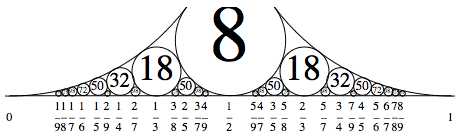
\includegraphics[scale=.8]{Ford-circles.png} 
\end{center}
\caption{Ford circles with tangent points and curvatures.
Recall that the curvature of a euclidean circle is the reciprocal of its radius.}
\end{figure}

The following is well known and is easily checked:

\begin{lem}\label{ford}
The Ford circle tangent to the real line at $m/n$
has Euclidean diameter $1/n^2$.
\end{lem}


We define the \textit{length} of the vertical line 
$\{ k/p + i t,\, t \in \RR \}$
to be the length of the  sub arc joining 
$F$ to the Ford circle tangent at $k/p$.
Further we define its  \textit{mid point} to be the midpoint of this sub arc.
We remark that if the projection of the line to $\xx$
is invariant by an automorphism 
then the midpoint is necessarily a fixed point of the automorphism.

The following is a restatement of Lemma \ref{ford} in terms of these notions:

\begin{lem}.\label{calcul}
Let $m/n$ be a rational. 
Then the geodesic $\{ m/n + i t,\, t \in \RR \}$
\begin{itemize}
\item has  length $2\log n$. 
\item has its midpoint at $ \frac{1 }{n}(m + i).$
\end{itemize}
\end{lem}

Finally, the key lemma that relates the $\sl2$ action to sums of squares is:

\begin{lem} \label{squares}
Let $n$ be a positive integer.
The number of  ways of writing $n$  as a  sum of squares
$$n = c^2 + d^2$$
with $c,d$ coprime integers
is equal to the number the  integers $0 \leq k < n-1$ coprime to $n$
such that the line
$$\{  k/n + i t,\, t \in \RR \}$$
contains  a point in the $\sl2$  orbit of $i$.
\end{lem}


\proof  Suppose there is such  a point which we denote  $w$.
The point $w$ is a fixed point of some  element of order 2 in $\sl2$.
Since the Ford circles are $\sl2$ invariant
this element must permute $F$ with the Ford circle tangent 
to the real line  at the real part of $w$.
So, in particular, $w$ is the midpoint of the line 
that it lies on 
and by  Lemma \ref{calcul} one has:

$$\frac{1}{n} = \im \frac{1 }{n}(k + i)  
= \im  \frac{ai +b}{ci+d }
= \frac{\im i} {c^2 + d^2}.$$

Conversely if $c,d$ are coprime integers 
 then there exists $a,b$ such that
 $$ad - bc = 1 \Rightarrow  
 \begin{pmatrix}
 a & b \\
 c & d
 \end{pmatrix} \in \sl2.
$$
%The real part of $w = \frac{ai +b}{ci+d }$ is
%$$ac + bd = (a,b).(c,d),$$
%and
By applying a suitable power of the parabolic transformation 
$z \mapsto z + 1$,
one can choose $w$ such that $0 \leq \text{Re\,} w < 1$.
So if $n = c^2 + d^2$ then $\frac{ai +b}{ci+d }$
is on one of the lines of the family in the statement.

\hfill $\Box$

\subsubsection{Cusp regions}

The image of a Ford circle on $\xx$ is a \textit{cusp region}
around one of the three cusps $0,1,\infty$.
It is not difficult to see that these cusp regions 
are permuted by the automorphisms of $\xx$.
It follows that if an automorphism preserves a geodesic  joining cusps on $\xx$
then it must permute the Ford regions at each end of a lift to $\HH$.

\subsection{The Group action}

Let  $K^0$ denote 
the subgroup of automorphisms 
that preserves the cusp labelled $0$ on $\xx$.
This group is generated by  automorphisms induced by the maps
$$U': z \mapsto 2-\bar{z},\, V' : z \mapsto \bar{z}/(\bar{z} - 1)$$
so that  their composition is 
$$U'\circ V' : z \mapsto z \mapsto (-z + 2) /( z + 1)$$
whose fixed point is $i+1$.


Now $K^0$ permutes the cusps labelled $\infty$ and $1$
and further:

\begin{lem} \label{action}
 The group $K^0$  permutes the geodesics of $\gg$.
\end{lem}
\proof
Let $g \in K^0$ and $\gamma \in \gg$ a geodesic.
Choose a lift $\tilde{g} : \HH \mapsto \HH$ of $g$.
By Lemma  \ref{calcul} the  length of any lift  $\hat{\gamma} \subset \HH$ is $2\log n$
and, since $\tilde{g}$ normalises $\g2$, it preserves the Ford circles
so that  $\tilde{g}(\hat{\gamma})$ has the same length.
Since $g(\gamma)$ joins the cusps labelled $\infty$ and $1$
there is a lift of this geodesic which is a vertical line
 and the other endpoint is a rational $m/n$.
The length of the lift  is again $2 \log n$ so
the diameter of this  Ford circle is $1/n^2$
and by Lemma \ref{ford} its center is a multiple of $1/n$.
\hfill $\Box$


 
 \section{Proof of Fermat's Theorem}

Throughout this section the integer $n$ is a prime which we denote $p$.
We can deduce Theorem \ref{main} from:

\begin{lem} \label{midpoint}
Let $p$ be a prime congruent to 1 or 2 modulo 4.
Then there is always a geodesic 
in the family $\ggp$
 that has as its  midpoint a point in the $\sl2$  orbit of $i$.
\end{lem}


This is equivalent to saying that, 
on projecting to the surface  $\xx$,
 there  is always a geodesic which passes through
the  fixed point of the map induced by $U'\circ V'$.

\subsection{The singular case of Lemma \ref{midpoint}}

The case $p=2$ is exceptional and we will deal with it first.
From the preceding paragraph there is a single geodesic namely 
the projection of the line 
$$\{ 1/2 + i t,\, t \in \RR \}$$
and this contains the point  $\frac{1}{2 }(1+ i)$
Note that one has 
$$\begin{pmatrix}
1 & 0 \\
1 & 1
\end{pmatrix} \in \sl2,\,\, \begin{pmatrix}
1 & 0 \\
1 & 1
\end{pmatrix}.i  = \frac{1}{2 }(1+ i)$$
so this point is in the $sl2$ orbit of $i$>
Then one has as in Lemma \ref{squares}:
$$\im \frac{1}{2 }(1+ i) = \frac{1}{2}  =  \im \begin{pmatrix}
1 & 0 \\
1 & 1
\end{pmatrix}.i = \frac{\im i}{ 1^2 + 1^2}$$
So, in a rather roundabout way, we obtain $2$ as a sum of squares by comparing denominators:
$$2 = 1^2 + 1^2.$$




\subsection{Inversions and fixed geodesics}

We will finish the proof of  Lemma \ref{midpoint}
by showing that there is a geodesic invariant by 
the orientation preserving automorphism in $K^0$,
obtaining the required midpoint as the fixed point of the automorphism.
Our  argument is exactly  the same as for
 Theorem \ref{triv}.
 More precislely, we show that, for $p > 2$:
\begin{enumerate}
\item the automorphism induced by $U'$ preserves no geodesic in  $\ggp$
\item the automorphism induced by $V'$ preserves at most two geodesics in $\ggp$
\end{enumerate}

%\subsubsection{Conjugations between  inversions}
The first point is rather easy 
(the automorphism induced by $U'$ fixes three disjoint geodesics joining 
cusps and permutes the pair of ideal triangles in their complement)
 but the second requires establishing
 the analogue of the fact that  the equation
$$x^2 = 1$$
has at most two solutions in any field or integral domain for that matter. 
Let us start by saying which geodesics are preserved 
by the automorphism: they are unsurprisingly the pair with endpoints $\pm 1/p$.
To see this consider the map
\begin{equation}
\label{inversion}
z \mapsto \frac{\bar{z}}{ p\bar{z} - 1},
\end{equation}
and observe that on setting $p=1$ the resulting map coincides with $V'$.
This map fixes $0$ and $2/p$ and permutes $1/p$ and $\infty$
 so that it maps the geodesic of $\hat{\gg}$ with endpoint $1/p$ to itself.
 Moreover the map  is an inversion in the semi circle joining $0$ and $2/p$  
and is conjugate to $V'$ by an element of $\g2$. 
The following is an elementary exercise in (hyperbolic) geometry:

\begin{lem}\label{fps}
Let $\phi_1$ (resp. $\phi_2$)
 be an of inversion of $\HH$ with fixed point set
  $L_1  \subset \dHH$ (resp $L_2$).
Then $\phi_1$ and $\phi_2$
  are conjugate by an isometry  $f$ 
  (i.e. $\phi_1 = f\circ \phi_2 \circ f^{-1}$)
  if and only if $ f(L_1) = L_2.$
\end{lem} 
%( via an element of $\g2$ if $(p-1)2$ is even.)
So it suffices to find a  map that takes one fixed point set to the other.
To do this it proves convenient to represents the fixed point set, 
which is a geodesic in $\HH$,
by its endpoints, which are a pair of rational numbers,
and encode this pair as a matrix 
whose entries are  the numerators and denominators of the fractions..
Concretely, to an ordered  pair of rationals  $(m/n, m'/n')$ , 
 we associate the following matrix:
$$\begin{pmatrix}
m & m'\\
n & n'
\end{pmatrix}.
$$
%This matrix represents the geodesic joining $m/n$ to $m'/n'$.
Determining the  conjugation in Lemma \ref{fps}
is reduced to solving a matrix equation.
For example, for the pair $0/1, 2/1$  and  $0/1, 2/p$   one has the matrix equation:
\begin{equation}
\begin{pmatrix}
0 & 2\\
1 & 1
\end{pmatrix}
= 
\begin{pmatrix}
1 & 0 \\
 -(p-1)/2& 1\\
\end{pmatrix}
\begin{pmatrix}
0& 2\\
1 & p
\end{pmatrix}.
\end{equation}
The first factor of the LHS is an element of $\g2$ iff $(p-1)/2$ is even
 and from it, using Lemma \ref{fps}, we can obtain an isometry of
$\HH$ conjugating the inversion (\ref{inversion}) to $V'$.

Conjugating the map defined in (\ref{inversion}) above
by $z \mapsto z + 1$ 
one obtains an inversion 
which permutes $\infty$ and  $1 + 1/p$.
It follows that  geodesic in $\gg$ with endpoint $1 + 1/p$ 
projects to a second geodesic on $\xx$
preserved by the automorphism induced by $V'$.

%We say that a pair of (extended) rational $m/n, m'/n'$ are \textit{Farey neighbors} 
%if $|mn' - nm'| = 1$ with the convention that $\infty = 1/0$ 
%so that it's neighbors are exactly the integers $m/1$.
%The Farey neighbors of $0= 0/1$ are the rationals $1/n$ and in particular $1/p$ 
%is one of them though $2/p$ is not. 


\subsection{Exactly two fixed geodesics.}

Having established the existence of suitable geodesics in the preceding paragraph
it suffices to show that no other geodesic is preserved.


\begin{lem} \label{the end}
Let $p$ be a prime.
The automorphism induced by $V'$ preserves two and exactly two geodesics in $\ggp$.
\end{lem}


\proof 
We give a proof for  $p$ be a prime congruent to 1 modulo 4
the proof of the other case is similar.

Let $1< k < p-1$  be an integer. 
It suffices to show that the inversion in the semi circle with endpoints  
 $(k-1)/p$ and  $(k+1)/p$
(i.e. the one that permutes $F$ and the Ford circle tangent at $k/p$)
is not conjugate to $V'$ 
via a hyperbolic isometry induced by an element of $\sl2$.
Consider the  matrix equation we must solve 
to find the required element of $\sl2$:
\begin{equation}
\begin{pmatrix}
0& 2\\
1 & 1
\end{pmatrix}
= 
\begin{pmatrix}
a & b \\
c & d\\
\end{pmatrix}
\begin{pmatrix}
k + 1 & k-1 \\
p  & p
\end{pmatrix}.
\end{equation}

Suppose that a solution exists. Taking determinants one obtains a contradiction immediately:
$$ 2 = 1 \times 2p \Rightarrow p = 1.$$

\hfill $\Box$


\subsubsection{Non prime integers}

It is well known that the set of integers $n$ 
which can be written as a sum of squares 
$c^2 + d^2$ with $c,d$ co prime is closed under multiplication.
For example one has
$$50 = 5^2 \times 2 = | (1+2i)^2 (1+i) |^2 = |  -7 + i |^2 = 7^2 + 1^2 $$
and
$$65 = 5 \times 13 = | (1+2i)(2+3 i) |^2 = |  -4 + 7i |^2 = 7^2 + 4^2.$$
It seems difficult to prove this directly by considering 
the set $X$ of bi cuspidal  geodesics of length $2\log 65$.
The Burnside Lemma for the group of automorphisms we consider above yields:
$$4 |X/G|   = \phi(65)+  |\{ x, x^2 = 1 \}| + |\{ x, x^2 = -1 \}| = 48 + 4 +  |\{ x, x^2 = -1 \}|.$$
It is easy to check that the 
kernel of the morphism 
$$x \mapsto x^2,\, (\ZZ/65)^* \rightarrow (\ZZ/65)^*$$
acts on the orbit space $X/G$
and from this one can deduce that $|X/G|$ is even.
It is an immediate consequence that 
$$ 4 +  |\{ x, x^2 = -1 \}| = 0 \mod 8 $$
so $x^2 = -1$ 
has solutions in $(\ZZ/65)^*$
(these are precisely  $8,18,47,57$.)
In fact $65$ can be written as a sum of two  squares 
in two essentially different ways towit
$$ 65 =  7^2 + 4^2 = 8^2 + 1.$$
It seems likely that this kind of argument,
that is showing $|X/G|$ is divisible by some power of $2$,
can be adapted to the geometric setting to show this.


\section{\thebibliography{99}}

\bibitem{aigner}
M. Aigner
\textit{Markov's Theorem and 100 Years of the Uniqueness Conjecture}, Springer( 2013)

\bibitem{barag}
A. Baragar,
\textit{On the Unicity Conjecture for Markoff Numbers}
Canadian Mathematical Bulletin , Volume 39 , Issue 1 , 01 March 1996 , pp. 3 - 9

\bibitem{button}
J. O. Button, 
\textit{The uniqueness of the prime Markoff numbers},
 J. London Math. Soc.
(2) 58 (1998), 9–17.

\bibitem{cana}
Ilke Canakci, Ralf Schiffler
\textit{Snake graphs and continued fractions}
European Journal of Combinatorics
Volume 86, May 2020, 103081


\bibitem{ford}
Lester R Ford,
\textit{Automorphic Functions}

\bibitem{thesis}
G. McShane,
\textit{Simple geodesics and a series constant over Teichmuller space}
Invent. Math. (1998)

\bibitem{mong}
M.L. Lang, S.P Tan,
\textit{A simple proof of the Markoff conjecture for prime powers}
Geometriae Dedicata volume 129, pages15–22 (2007)

\bibitem{bob}
R. C. Penner, 
\textit{The decorated Teichmueller space of punctured surfaces}, 
Communications in Mathematical Physics 113 (1987), 299–339.





\bibitem{serre}
J-P. Serre,
\textit{A Course in Arithmetic},
Graduate Texts in Mathematics,
Springer-Verlag New York
1973

\bibitem{saw}
Scott Wolpert,
\textit{On the Kahler form of the moduli space of once-punctured tori}, 
Comment. Math. Helv. 58(1983)246-256

\bibitem{zagier}
D. Zagier,
 \textit{A one-sentence proof that every prime p = 1 (mod 4) is a sum of two squares}, 
 American Mathematical Monthly, 97 (2): 144
 
 \bibitem{zhang}
 Y. Zhang,
 \textit{ An elementary proof of uniqueness of Markoff numbers}
 preprint, arXiv:math.NT/0606283
 
  \bibitem{zhang2}
   Y. Zhang,
 \textit{Congruence and uniqueness of certain Markoff numbers}
 Acta Arithmetica, Volume: 128, Issue: 3, page 295-301




%\bibitem{mcp}
%Greg McShane, Hugo Parlier,
%Multiplicities of simple closed geodesics and hypersurfaces in Teichmüller space,
%Geom. Topol.
%Volume 12, Number 4 (2008), 1883-1919.
%
%\bibitem{mcr}
%Greg McShane, Igor Rivin
%\textit{A norm on homology of surfaces and counting simple geodesics}
%International Mathematics Research Notices, Volume 1995, Issue 2, 1995
%
%
%
%\bibitem{ra}
%M. Rabideaua, R. Schiffler,
%\textit{Continued fractions and orderings on the Markov numbers},
%Advances in Mathematics Vol 370,  2020.
%
%
%
%\bibitem{vu}
%C Lagisquet and E. Pelantová and S. Tavenas and L. Vuillon,
%\textit{On the Markov numbers: fixed numerator, denominator, and sum conjectures.}
%\url{https://arxiv.org/abs/2010.10335}
%


%\bibitem{Gui}
%L. Guillop\'e, Laurent(F-GREN-F)
%Sur la distribution des longueurs des g\'eod\'esiques ferm\'ees d'une surface compacte \`a bord totalement g\'eod\'esique. 
%Duke Math. J. 53 (1986), no. 3, 827-848. 

%\bibitem{MC}
%C. L. Mallows and J. M. C. Clark. 
%{\it Linear-intercept distributions do not characterize plane sets}
% Journal of Applied Probability, 7(1):240-244, 1970.
% 
% \bibitem{Masai-McShane}
% Masai, Hidetoshi and Greg McShane,
% ``On systoles and ortho spectrum rigidity'', preprint.
% \bibitem{MMc}
% Masai, Hidetoshi, and Greg McShane. "Equidecomposability, volume formulae and ortho spectra." Algebraic \& Geometric Topology 13.6 (2013): 3135-3152.
 



\end{document}


For the pair $\infty, 1/2$  and  $0, 2/p$   one has the matrix equation:
\begin{equation}
\begin{pmatrix}
1 & 1\\
0 & 2
\end{pmatrix}
= 
\begin{pmatrix}
 -(p-1)/2& 1\\
1 & 0
\end{pmatrix}
\begin{pmatrix}
0& 2\\
1 & p
\end{pmatrix}.
\end{equation}


The first matrix on the LHS is an element of $\gl2$
and from it, using Lemma \ref{fps}, we can obtain an orientation reversing isometry of
$\HH$ conjugating the inversion (\ref{inversion}) to $V$.
Finally, by changing signs in the expression(\ref{inversion})  one obtains an inversion 
conjugate to $V$ mapping the geodesic with endpoint $-1/p$ to itself.

%We say that a pair of (extended) rational $m/n, m'/n'$ are \textit{Farey neighbors} 
%if $|mn' - nm'| = 1$ with the convention that $\infty = 1/0$ 
%so that it's neighbors are exactly the integers $m/1$.
%The Farey neighbors of $0= 0/1$ are the rationals $1/n$ and in particular $1/p$ 
%is one of them though $2/p$ is not. 
